\section{模型的适用范围}
\label{sec:cprob-scope}

古典模型的全部计算都建立在一个前提上：样本空间有限，每个样本点同样可能。前面几节一再看到，同一个试验换一种记录方式，这个前提就可能不再成立。本节把失效的情形归为三类：记录合并了不等量的基本结果、结果有无穷多个、结果取连续的位置。对每一类，我们说明计数比为什么失效，以及后面的章节用什么代替它。

\paragraph{合并后的结果}
掷两枚骰子，如果只记录出现了哪两个点数而不分先后，结果就是可重复的无序对，例如$\{1,1\}$、$\{1,2\}$、$\{3,5\}$。由表~\ref{tab:cprob-sampling}最后一行，这样的结果共有$\binom{6+2-1}{2}=21$个。它们是否同样可能？

图~\ref{fig:cprob-merged-classes}显示了每个无序结果合并了哪些有序结果。对角线上的$\{i,i\}$只对应一个有序对$(i,i)$，概率是$1/36$；其余的$\{i,j\}$（$i\neq j$）对应关于对角线对称的两个格子$(i,j)$与$(j,i)$，概率是$2/36$。$6$个一类、$15$个另一类，验证总和：
\[
 6\times\frac{1}{36}+15\times\frac{2}{36}=\frac{36}{36}=1.
\]

\begin{BookInlineFigure}
  \centering
  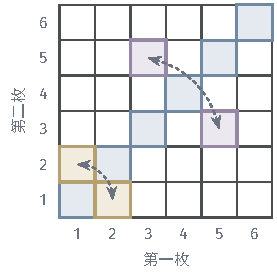
\includegraphics[width=47mm]{figures/07-probability/01-elementary-probability/tikz/cprob-merged-classes/figure.pdf}
  \caption{不记次序时两枚骰子的结果。浅蓝的对角线格子各自构成一个无序结果$\{i,i\}$；其余无序结果各由关于对角线对称的两个格子组成，黄色一对是$\{1,2\}$，紫色一对是$\{3,5\}$，虚线连接同一结果的两个格子。}
  \label{fig:cprob-merged-classes}
\end{BookInlineFigure}

若直接在$21$个无序结果上数，“两枚点数相同”占$6$个，会得到$6/21=2/7$；正确的答案是$6/36=1/6$。错误不在于用无序记录，而在于把合并了不同数量基本结果的类别当成了等可能的点。

一般地，若一个结果$r$是若干个等可能基本结果合并而成的，它的概率等于所合并的基本结果的概率之和。合并的个数不同，各结果的概率就不同。这时仍可以计算，但要给每个结果单独记一个概率$p(r)\geq0$，所有$p(r)$之和为$1$，事件的概率是它所含结果的$p(r)$之和。摸球的颜色记录、点数和、无序的点数对都属于这种情形，第~\ref{sec:cprob-equally-likely}节的三条基本性质对这样的分配仍然成立。

有些试验根本没有一个等可能的细化。一枚重心偏移的骰子，六个面朝上的机会本来就不同，无论怎样细分记录都找不到对称性。古典模型对它无能为力，只能直接给六个面各指定一个概率。给有限或可数个结果逐一指定概率的方式称为概率表，它在第~\ref{chap:random-variables}章与随机变量一起建立。

\paragraph{无穷多个结果}
抛一枚均匀硬币，直到第一次出现正面为止，记下所抛的次数。结果可以是$1,2,3,\ldots$中的任何一个，样本空间$\Omega=\{1,2,3,\ldots\}$有无穷多个点。

这些结果不可能同样可能。若每个结果的概率都是同一个数$c$，那么$c>0$时，任意取$N>1/c$个结果，它们的概率之和就超过$1$；$c=0$时，所有结果的概率都是零，总和无法是$1$。计数比$\lvert A\rvert/\lvert\Omega\rvert$在这里更没有意义，分母是无穷。

各结果的概率可以从有限的古典模型中算出。“第一次正面出现在第$k$次”只与前$k$次有关，它要求前$k-1$次都是反面、第$k$次是正面。前$k$次的$2^{k}$个有序结果等可能，满足要求的只有一个，所以
\begin{equation}
 \mathbb{P}(\text{第一次正面出现在第}k\text{次})=\frac{1}{2^{k}},\qquad k=1,2,\ldots.
 \label{eq:cprob-first-head}
\end{equation}

图~\ref{fig:cprob-first-head}(a)画出这些概率，它们随$k$成倍减小。前$k$项之和是$1-2^{-k}$，见图~\ref{fig:cprob-first-head}(b)，它随$k$增大而趋于$1$，但任何有限项之和都小于$1$。要让总概率等于$1$，必须把无穷多个结果的概率加起来，这要求可加性从有限个事件推广到可数个事件。

\begin{BookInlineFigure}
  \centering
  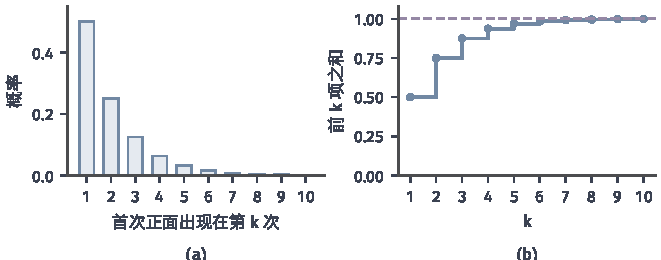
\includegraphics[width=112mm]{figures/07-probability/01-elementary-probability/matplotlib/cprob-first-head/figure.pdf}
  \caption{抛硬币直到第一次正面。(a)第一次正面出现在第$k$次的概率$2^{-k}$；(b)前$k$项之和$1-2^{-k}$，紫色虚线是总和$1$，有限项之和都达不到它。}
  \label{fig:cprob-first-head}
\end{BookInlineFigure}

\paragraph{连续的位置}
在长为$1$的木棍上随机选一个点，点的位置可以是$[0,1]$中的任何实数。所谓“随机”，自然的意思是长度相同的两段被选中的机会相同。问点落在$(0.2,0.5]$中的概率是多少？

计数比在这里给不出答案：$(0.2,0.5]$与$[0,1]$都有无穷多个点，比值是“无穷比无穷”。可以先用有限模型逼近：在$(0,1]$上取$n$个等距位置$k/n$，$k=1,\ldots,n$，让它们等可能。这是一个古典模型，事件“落在$(0.2,0.5]$中”的概率是其中位置的个数除以$n$。

图~\ref{fig:cprob-grid-uniform}(a)显示，随着$n$增大，这个计数比趋于区间的长度$0.3$。例如$n=10$时恰有$3$个位置，比值是$0.3$；$n=7$时有$k=2,3$两个位置，比值是$2/7\approx0.286$。另一方面，图~\ref{fig:cprob-grid-uniform}(b)中单个位置的概率$1/n$趋于$0$。

\begin{BookInlineFigure}
  \centering
  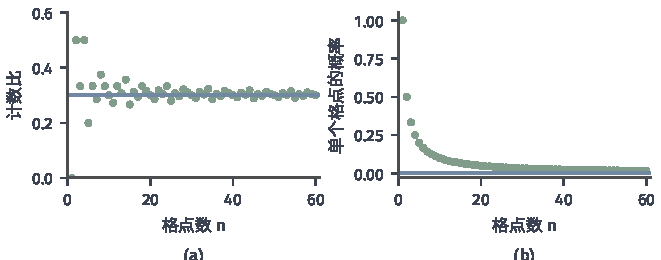
\includegraphics[width=112mm]{figures/07-probability/01-elementary-probability/matplotlib/cprob-grid-uniform/figure.pdf}
  \caption{用$n$个等距位置$k/n$逼近木棍上的随机点。(a)绿点是事件“落在$(0.2,0.5]$中”的计数比，蓝线是区间长度$0.3$；(b)绿点是单个位置的概率$1/n$，趋于蓝线$0$。}
  \label{fig:cprob-grid-uniform}
\end{BookInlineFigure}

这两个极限提示了连续情形的做法：区间的概率由长度给出，不由点数给出；每个单点的概率都是$0$，但每个点都可能被选中。概率为零不等于不可能，这在有限的古典模型中不会发生，那里$\mathbb{P}(A)=0$当且仅当$A=\varnothing$。长度的作用在一般情形中由密度承担，单位长度上的概率可以随位置变化，第~\ref{chap:random-variables}章用积分计算这类概率。

\paragraph{三类情形的统一}
表~\ref{tab:cprob-models}把本节的几种情形放在一起。它们分配概率的方式不同，但都应当满足非负、总量为$1$、互斥事件的概率相加这几条要求；可数个结果和连续位置还要求可加性对可数个互斥事件成立。

\begin{BookInlineTable}
  \centering
  \caption{几类概率模型分配概率的方式}
  \label{tab:cprob-models}
  \begin{tabular}{lll}
    \toprule
    样本空间 & 例子 & 事件的概率 \\
    \midrule
    有限，等可能 & 均匀骰子、摸球 & 计数比$\lvert A\rvert/\lvert\Omega\rvert$ \\
    有限，不等可能 & 点数和、偏心骰子 & 所含结果的概率之和 \\
    可数无穷 & 首次正面的次数 & 所含结果的概率之和（级数） \\
    连续位置 & 木棍上的点 & 长度，一般为密度的积分 \\
    \bottomrule
  \end{tabular}
\end{BookInlineTable}

把这些情形纳入同一个框架，需要回答哪些集合可以作为事件、概率怎样对可数个事件相加，以及长度这样的量能定义在哪些集合上。这些问题在第~\ref{chap:probability-spaces}章用概率测度统一回答。在此之前，第~\ref{chap:random-variables}章先用概率表和密度直接处理有限、可数与连续的情形。
